\section{Bilan de la gestion du temps}
\label{sec:time}

Nous avons géré la planification avec les mêmes outils que nous avons présentés en décembre. Nous avons donc utilisé le gestionnaire de version Git. Nous utilisions d'ailleurs le Gitlab fourni par l'INSA. Nous communiquions par Skype afin de discuter des tâches à réaliser et des problèmes rencontrés. Enfin, pour le suivi des tâches, nous utilisions le modèle Excel fourni par Yoann Royer que nous disposé sur le Google Drive mis en place pour le projet. Celui-ci nous permettait de visualiser les différentes tâches ainsi que les personnes auxquelles elles sont assignées et le nombre d'heures qu'elles ont passées dessus. Nous avions ainsi un résumé rapide du travail accompli entre chaque réunion. La liste des tâches était basée sur la planification que nous avons fait sur Microsoft Project. Cependant, cette dernière manquait de détails, nous l'avons complétée et mise sur le document Excel de suivi des tâches. Ainsi, ces dernières étaient accessibles pour tout le monde et facilement modifiables. 

\subsection{Bilan par rapport à la planification initiale}

Notre planification initiale réalisée en décembre 2015 prévoyait 946h de temps de travail pour le projet dont 479h pour le second semestre. Nous l'avions basée sur 8h de travail par personne par semaine. La figure \ref{CamFirst} montre la répartition horaire dans chaque partie du projet prévue lors de la planification initiale.

    \begin{figure}[H]
        \centering
        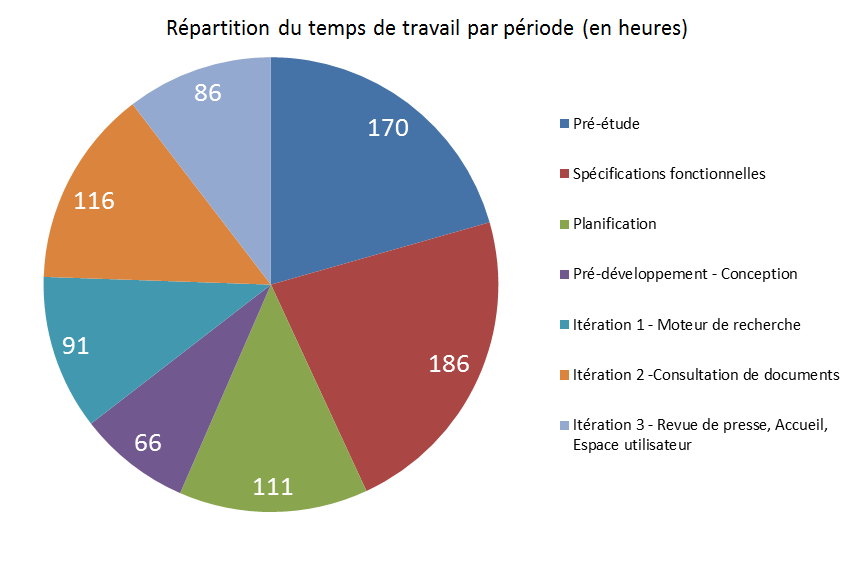
\includegraphics[width=\textwidth]{figure/camembertfirst.png}
            \caption{Graphique représentant la répartition horaire initialement prévue}
            \label{CamFirst}
    \end{figure}

Au final, nous arrivons à 408h de travail réalisées avec environ 6h de travail par personne par semaine. Nous avons un nombre d'heures plus bas que l'estimation principalement parce que nous avions surestimé certaines tâches et qui se sont avérées plus simples à réaliser grâce notamment aux divers frameworks et bibliothèques auxquels nous avons fait appel. Cependant, la figure \ref{Camsec} qui montre la répartition finale de chaque partie, nous permet de constater que cette surestimation concernait principalement les itérations 1 et 2. En effet, la tâche nous facilité notamment par l'utilisation respectivement d'Elasticsearch et OpenSeadragon qui nous ont permis d'arriver plus facilement à une solution viable. De même, l'itération 3 contient aussi les modifications et ajouts par rapport à l'itération 2 et ces derniers ont été plus nombreux que sur les autres itérations ; nous avons même ajouté certaines fonctionnalités auxquelles nous n'avions pas pensé dans les spécifications. 

	\begin{figure}[H]
        \centering
        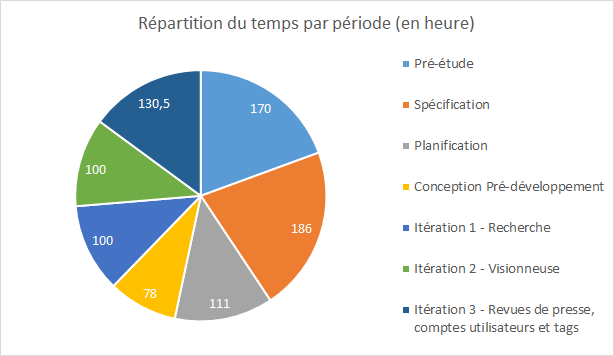
\includegraphics[width=\textwidth]{figure/camembertsecond.png}
            \caption{Graphique représentant la répartition horaire finale}
            \label{Camsec}
    \end{figure}

\subsection{Bilan des itérations}

La figure \ref{grapheHeure} montre le nombre d'heures réalisées par semaine tout au long du projet avec les dates des différents rendus. 

	\begin{figure}[H]
        \centering
        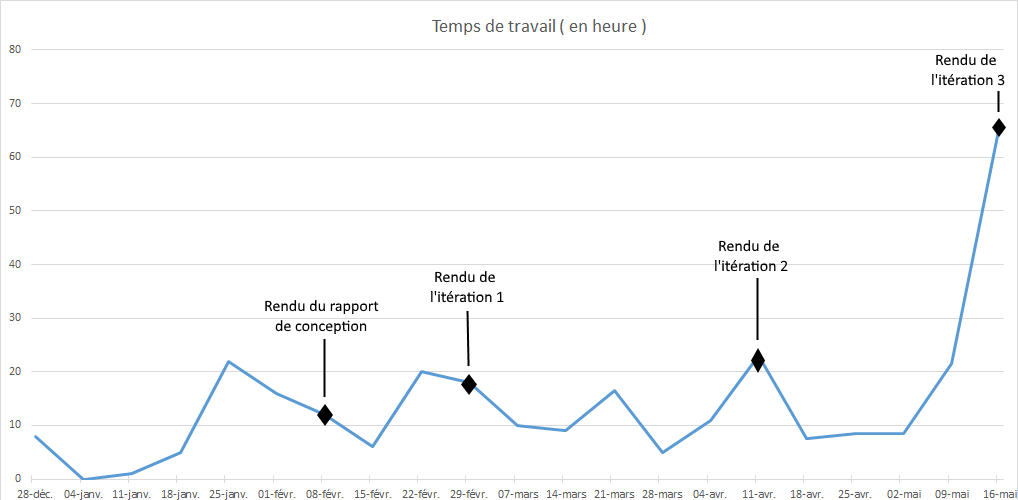
\includegraphics[width=\textwidth]{figure/iteration.png}
            \caption{Graphique représentant le nombre d'heures réalisées par semaine durant le projet}
            \label{grapheHeure}
    \end{figure}


On peut constater que le développement de l'application ne se faisait régulière notamment à cause des différents rendus et devoirs surveillés que nous avons dans les autres enseignements.  


Nous avons aussi eu des retards au niveau des rendus des itérations. D'abord, pour la première, à cause de tâches indiquées trop vagues, certains d'entre nous n'avaient pas totalement compris ce qui était exigé derrière ces tâches. Par conséquent, à la fin de l'itération 1, les tâches n'étaient réalisées que partiellement. Pour la deuxième itérations, nous avons donc corrigé cela en décomposant les grandes en plus petites qui sont alors plus précises. Nous avons alors rendu, cette fois, tous ce qui étaient exigés pour cette itération mise à part une fonctionnalité. Quant à la troisième, le rendu était le mardi de la première semaine bloquée de mai. Cependant, nous avons eu besoin de toute la semaine bloquée ainsi que du weekend pour terminer cette itération car, entre autres, l'une des personnes de notre groupe s'est absentée depuis peu avant la semaine bloquée, ce qui nous a beaucoup handicapé pour cette fin d'itération.      